% !TEX root = main.tex

\section{Introduction}

No single radio design or set of wireless protocols can meet the specific needs and constraints of the many applications for wireless technology.  As a result, heterogeneity has become a fundamental property of the wireless spectrum.  Differences in physical layers, MAC layers, transmission powers, and spectral bandwidths are driven by these varying application requirements.  Unfortunately, differences in these properties break down spectrum sharing and can lead to significant interference between heterogeneous technologies~\cite{buzzbuzz,wifinet,airshark,rfsmog}. 

One popular approach to prevent such heterogeneous interference is to develop coexistence techniques between pairs of technologies (e.g., between Wifi and ZigBee~\cite{buzz buzz}, or Cordless Phones and Wifi~\cite{rfsmog}). While coexistence techniques can alleviate interference, this general approach requires $N^2$ solutions between all technology pairs (where $N$ is growing).  Additionally, coexistence techniques are difficult to deploy.  They incur overhead, changes are often needed at lower layers (e.g., PHY \& MAC), and rapid changes to  technologies and standards can make such solutions short-lived.

% require modifications to layers that are implemented in the radio hardware (e.g., PHY \& MAC), they can , they incur overhead and complexity, and they are short lived due to wireless technologies rapidly changing.  
 
To the contrary, \emph{heterogeneous spectrum management can be an efficient and long-term solution}.  Ideally, the approach frequency-isolates incompatible technologies when possible, and otherwise intelligently places them together where they will receive and generate the least interference.  This approach has several key benefits:  1) It does not require changes to the protocols or radios, 2) It is a ``single solution'' (i.e., it does not require a unique solution/technique for each pair of technologies), and 3) It can continue to be applied to future technologies if the model is generic.

% If modeled and applied generically (i.e., without specifics to any single technology), the approach can 
%
%does not incur overhead, require pairwise solutions, and 
%
%While this approach can have greater longevity, it is non-trivial
%
%While we have made strides in gathering the required information about heterogeneous radios and their interference (e.g., through monitors such as Airshark, DOF, RFDump, and WifiNet \cite{airshark,dof,rfdump,wifinet}), \emph{our spectrum assignment models and algorithms are predominantly homogeneous and Wifi-centric}. 
%
%
%At the most basic level, spectrum management has required information about where signals go and what they interfere with.

Recently, monitors such as Airshark, DOF, RFDump, and WifiNet \cite{airshark,dof,rfdump,wifinet} have made strides in gathering the required environmental information about heterogeneous radios and their interference which makes spectrum management possible.  \emph{However, our spectrum assignment models and algorithms are predominantly homogeneous and Wifi-centric, unable to represent and use such information to efficiently (re)assign heterogeneous spectrum.}  



%For example, historical models such as graph coloring~\cite{utilfair,unified} are unable to represent differences in MAC layers and differences in spectrum usage (i.e., bandwidths and channels).  Referring to Figure~\ref{fig:color_example}, we show two possible ways to color a set of Wifi and ZigBee channels.  In \emph{Scenario 1}, all possible sets of channels (independent of technology) are given different colors.  When applying this scenario, traditional coloring algorithms will distribute ZigBee networks within Wifi channels under the assumption that they do not conflict (they have different colors).  This is agnostic to their destructive MAC interaction.  In \emph{Scenario 2}, if one colors all channels in the spectrum block the same (independent of bandwidth), the algorithm cannot properly distribute the sub-channels (e.g., ZigBee's, which have the same color).
%
%\begin{figure}[t]
%\centering
%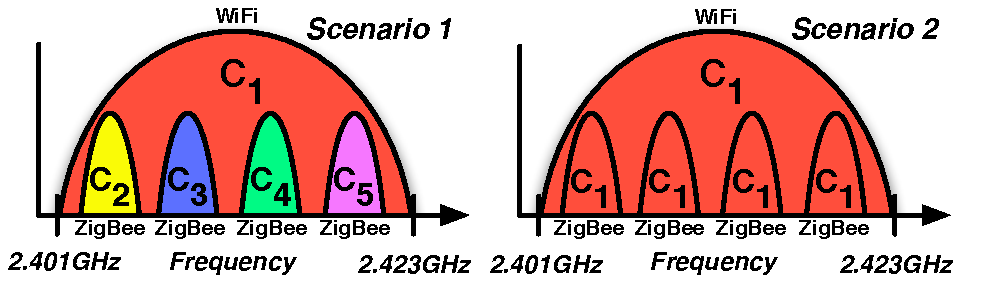
\includegraphics[width=3in]{figures/coloring_single}
%\vspace{-0.2in}
%\caption{\label{fig:color_example} \small Historical spectrum assignment models break-down under heterogeneity, as we illustrate with this graph coloring example.}
%\center
%\vspace{-0.3in}
%\end{figure}


%asymmetric power relationships, or the effects of differences in MAC layers, as commonly found 
%
%For example, historical models such as graph coloring cannot represent 
%
%%For example, graph coloring is unable to model 
%
%%As antidotal evidence, consider spectrum management between 
%
%For example, historical models such as graph coloring 
%
%Historical models such as graph coloring are unable to represent the critical differences in heterogeneous networks.  For example, whether 

%However, spectrum assignment models have remained fairly homogeneous and Wifi-centric.

%This requires knowledge of which heterogeneous devices are within range of each other in the environment, and a spectrum assignment model which, using such information, (re)organizes devices in the spectrum towards better efficiency.

%:  1)  Heterogeneous and spatial information about the environment, i.e., where heterogeneous signals go and what they interfere with, and 2)  A spectrum assignment model that is \emph{accurate} and \emph{general} enough to be applicable to many technologies that consistently evolve.

%An ideal heterogeneous spectrum assignment model should be:  1) \emph{Generic} such that it is not tied heterogeneous spectrum assignment model needs to:  1)  

More recent work, albeit heterogeneous, remains Wifi-centric: non-Wifi transmitters are treated as static interferers, their interference is estimated on the Wifi network, and Wifi channels can be re-assigned (e.g., WifiNet~\cite{wifinet}).  Interference is \emph{not} estimated between all pairs of heterogeneous networks, and management only occurs on the Wifi network.

An ideal model needs to be able to represent differences in properties of heterogeneous networks and devices, it needs to be comprehensive (i.e., not Wifi-centric), and importantly: it should be \emph{generic, yet descriptive}.  In being generic, the model should not include specifics of technologies (e.g., of Wifi or Bluetooth); it should only use primitives e.g., \emph{is device X in range of Y, and does it coordinate with Y?}  In being descriptive, the model must support an accurate description of the environment and devices in it.  For example, the supported spectrum bands of devices and networks, their various bandwidths, and whether or not they can be reconfigured.

In this paper, we present a spectrum assignment model that is able to accurately represent heterogeneous environments and increase 

 believe meets these requirements and is generic enough to be applicable to a wide range of wireless technologies over time.  Our model is built around a database of information about heterogeneous networks and devices in the environment, collected by current heterogeneous monitoring systems~\cite{airshark,dof,rfdump,wifinet}.

%
%
%, and more recent work (e.g., WifiNet) focus on the sustained interference of Wifi
%
% For example, WifiNet can only estimate heterogeneous interference on a WiFi network (rather than an \emph{any-to-any} estimate), and lacks a model to organize the spectrum based on such measurements. As we will further describe, more traditional models (e.g., graph coloring) do not map well 

%generality and often remain extremely Wifi-centric (i.e., considering Wifi of highest priority in management).  
%
% (i.e., requirement 1), 
%
%A lack of heterogeneous monitoring has made such spectrum management difficult, recent strides in accurate heterogeneous monitors~\cite{airshark,dof,rfdump} can provide the information necessary for better spectrum management.  
%
%
%% that can minimize interference and provide better connectivity .  In fact, there has been a significant amount of work in developing heterogeneous monitors which can 
%
%The key challenges here are developing a spectrum management model that is applicable to heterogeneous environments where, as mentioned, there are many different properties
%
%a more applicable approach with greater longevity as technologies evolve is proper spectrum management.  The current state of spectrum management is unfortunately ``chaotic'' .  However, with the introduction of better heterogeneous monitors (e.g., Airshark~\cite{airshark}), we can now sense .
%
%We find that many traditional spectrum management techniques (e.g., graph coloring) do not apply well to heterogeneous environments, and a much more detailed model is needed to capture the many properties (we described above) that 
%
%We believe that, to , there needs to be a fundamental shift in focus from developing narrow 
%
% such techniques are often complex, incur overhead, and are short lived.  The protocols change rapidly
%
% We are seeing an increasing number of devices and protocols with diversity in bandwidths, physical layers (i.e., modulation), antenna designs, 
%
% No single radio design or set of wireless protocols (e.g., PHY \& MAC) can meet the specific needs and constraints of each application of wireless technology.  As a result, the wireless spectrum is populated 
%
%Unfortunately, such heterogeneity in the spectrum has proven to be a significant challenge.  
%
%Two popular approaches 
%
% As we find more applications for wireless technology, we are catering wireless protocols (e.g., PHY and MAC) and radios (e.g., transmission power)
%
%As a result, heterogeneity has become a fundamental property of the wireless spectrum. 
%
%To meet the specific needs and constraints of each application, we are catering the wireless protocols 
%
%More applications for wireless technology has increased the density in the spectrum significantly, and to meet the specific needs and constraints of each application we are catering the protocols and radios
%
%As we find more applications for wireless technology, we are catering the protocols and radio to the specific needs and constraints of the application.  
%
% that is increasing as we find more applications for wireless technology.  

%The demand for wireless technology to support a wide variety of applications (e.g., video streaming, sensor data), under a varying set of constraints (e.g., form factor, range, bandwidth) has lead to the development of an increasing number of wireless protocols.  No single protocol provides the highest performance for all applications while satisfying their various constraints.  
%
%This increase in protocol diversity, coupled with an impending ``spectrum crisis'' (i.e., where spectrum availability unable to meet demand)~\cite{fccbroadbandplan}, presents a critical challenge:  the coexistence of heterogeneous wireless networks.  The problem in their coexistence is that their protocol diversity breaks down proper coordination in spectrum sharing, thereby causing significant amounts of interference~\cite{11interf,rfsmog,buzzbuzz,airshark}.  Therefore, not only is the spectrum limited and demand on it is high, but access to it is becoming increasingly destructive.  
%
%Many approaches to this problem have been pair-wise solutions:  develop techniques to make protocol $A$ coexist with protocol $B$ (e.g.,~\cite{buzzbuzz,rfsmog,reactiveuser}).  Unfortunately, this approach requires $N^2$ solutions, typically focusing on one protocol as the ``victim,'' and the longevity of such solutions are short-lived.   Proposed techniques can require significant complexity (e.g., MIMO-based transmitters using cancellation~\cite{rfsmog}), and even significant amounts of infrastructure to simply detect sources of interference~(e.g., an enterprise environment of dual-radio APs running signature detection~\cite{wifinet}).
%
%Unfortunately, little work has been done as a whole to reduce interference between such
%
%In this paper, we take a novel approach to the problem of coexistence in a critical environment: the home.  

%Since heterogeneous networks have difficulty detecting and sensing each other, distributed spectrum organization typically fails in such environments.

